\section{DESA}
\label{sec:method}

\subsection{Method Overview}

Given an original query $q_o$, DESA generates a set of complementary
reference passages $R=\{r_1,\ldots,r_n\}$. Dense retrieval keeps the original
query as its base direction and adds only the new semantic component supplied
by the references. Sparse retrieval combines the original and expanded scores
so that generated terms can reorder documents already matched by the original
query without introducing expansion-only matches. The resulting Dense and
Sparse rankings are fused into the final result. Figure~\ref{fig:desa-overview}
summarizes this design: Dense expands; Sparse anchors.

\subsection{Complementary Evidence Generation}

The generator is prompted to produce $n$ short passages that could plausibly
occur in relevant documents. Each passage introduces a different alias,
technical term, or paraphrase while retaining the entities, relations,
numbers, polarity, temporal conditions, scope, and other constraints of
$q_o$. The prompt prohibits broader information needs and invented answers.
The passages therefore vary in expression rather than intent, allowing the
two retrieval channels to draw additional evidence from a shared expansion.
The complete prompt and decoding settings are provided in Appendix~A.

\newpage
\begin{figure}[t]
  \centering
  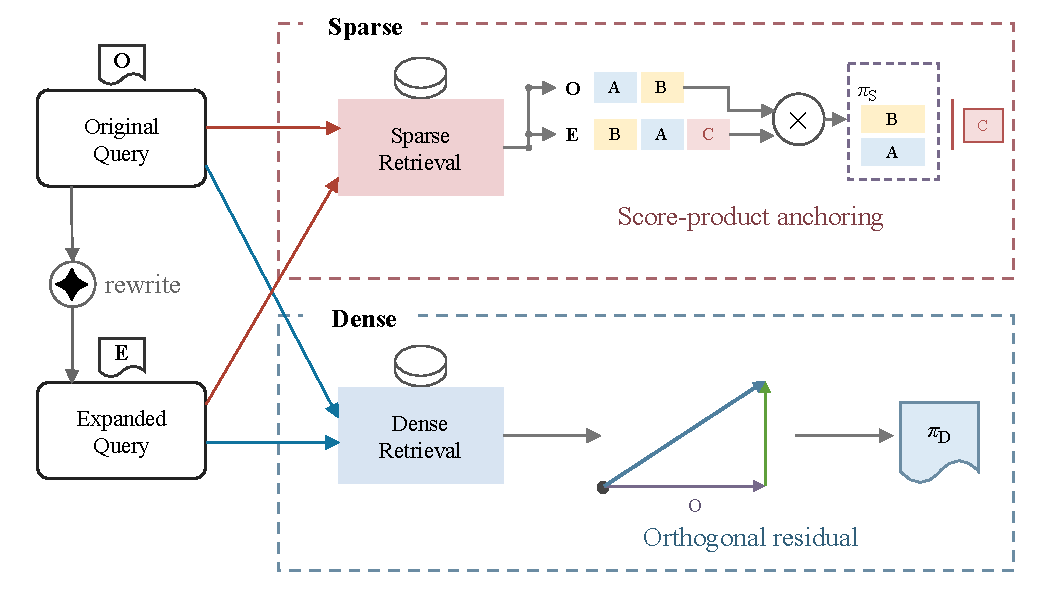
\includegraphics[width=\columnwidth]{figures/fig_desa_overview.pdf}
  \caption{Design principle of DESA. The same generated evidence expands
  Dense semantics but remains anchored to the original query's lexical support
  in Sparse retrieval.}
  \label{fig:desa-overview}
\end{figure}

\subsection{Channel-Asymmetric Query Construction}

\subsubsection{Orthogonal Residual Expansion}

Let $f_D$ be the Dense encoder. We encode the original query and each
query--reference pair as unit vectors:

\[
\begin{aligned}
\mathbf v_o&=\operatorname{norm}(f_D(q_o)),\\
\mathbf v_i&=\operatorname{norm}
\!\left(f_D(\operatorname{concat}(q_o,r_i))\right),\\
\bar{\mathbf v}_r&=\frac{1}{n}\sum_{i=1}^{n}\mathbf v_i .
\end{aligned}
\]

The component of $\bar{\mathbf v}_r$ parallel to the original query is
removed, and the remaining residual is added to $\mathbf v_o$:

\[
\mathbf z=
\bar{\mathbf v}_r-
(\mathbf v_o^\top\bar{\mathbf v}_r)\mathbf v_o,
\qquad
\mathbf e_D=\operatorname{norm}(\mathbf v_o+\mathbf z).
\]

Documents are ranked by their similarity to $\mathbf e_D$, producing the
Dense ranking $\pi_D$. Because $\mathbf z\perp\mathbf v_o$ and
$\|\mathbf z\|\leq1$,

\[
\angle(\mathbf e_D,\mathbf v_o)
=\arctan\|\mathbf z\|
\leq\frac{\pi}{4}.
\]

The references can therefore add semantic directions absent from the original
representation while keeping the expanded query within $45^\circ$ of it. If
they contribute no orthogonal component, then $\mathbf e_D=\mathbf v_o$.

\subsubsection{Score-Product Anchoring}

For Sparse retrieval, the expanded query concatenates the original query and
all reference passages:

\[
q_r=\operatorname{concat}(q_o,r_1,\ldots,r_n).
\]

Let $s_S(q,d)$ be a non-negative additive Sparse scorer. Each document $d$
receives an original score, an expanded score, and their product:

\[
\begin{aligned}
s_o(d)&=s_S(q_o,d), &
s_r(d)&=s_S(q_r,d),\\
s_A(d)&=s_o(d)s_r(d).&&
\end{aligned}
\]

Because $q_r$ contains $q_o$, every document supported by the original query
is also supported by the expanded query. Hence,

\[
\operatorname{supp}(s_A)
=\operatorname{supp}(s_o)\cap\operatorname{supp}(s_r)
=\operatorname{supp}(s_o).
\]

Sorting the positive anchored scores produces the Sparse ranking $\pi_S$.
Generated terms may promote or demote documents within the original support,
but documents matched only by the expansion receive zero anchored score and
are excluded. If $s_r$ is merely a positive multiple of $s_o$, the original
Sparse order is unchanged; positive global score rescaling also leaves the
ranking invariant.

\subsection{Complete Fusion and Access Measurement}
\label{sec:quality-access}

We fuse the complete Dense and Sparse rankings using equal-weight reciprocal
rank fusion \citep{cormack-etal-2009-rrf}:

\[
F(d)=
\sum_{c\in\{D,S\}}
\frac{1}{\kappa+\operatorname{rank}_{\pi_c}(d)}.
\]

A document absent from a channel contributes zero. Sorting by $F(d)$, with
document identifiers breaking ties, defines the ordered target $T_K$.
Retrieval effectiveness is evaluated directly on this complete-list result.

To measure channel access, a fixed replay procedure progressively reveals
$\pi_D$ and $\pi_S$. After $L_c$ items have been read from channel $c$, the
largest possible contribution from its next unread item is

\[
u_c(L_c)=\frac{1}{\kappa+L_c+1}.
\]

The replay reads from the channel with the larger bound, breaking ties in
favor of Dense, until the membership and order of $T_K$ can no longer be
changed by unread documents. It then records the Dense and Sparse depths
$(L_D,L_S)$, which quantify how much ranked evidence each channel must reveal
to determine the complete-list result.
